\chapter{Theoretical Foundations}

\section{The Simple Parton Model}

Over the past century studies of spin in elementary particle physics have proven
their worth time and again, exposing weaknesses in theories that were otherwise
able to explain the measurements of the day. The first indication that the
proton was itself a composite particle came from a spin experiment, namely
Stern's discovery that the magnetic moment of the proton is incompatible with
the Dirac prediction for spin-\(\frac{1}{2}\) particles. As a result, the
\textit{structure function} was introduced in scattering cross sections to
codify our lack of knowledge about the true internal structure of the nucleon.

In 1964, Gell-Mann and Zweig independently proposed models
\cite{GellMann:1964nj, Zweig:1964jf} in which hadrons are composed of a set of
point-like elementary particles. These models provided a convenient taxonomy for
the zoo of particles which had been identified in experiments, but it was
unclear whether the ``quarks'', to use Gell-Mann's term, represented actual
physical entities. Five years later, Feynman and Bjorken and Paschos postulated
that the quarks -- they called them partons -- would behave quasi-free at high
energies \cite{Feynman:1969ej, Bjorken:1969ja}. A consequence of this model is
that in the high energy limit the structure functions of the proton measured in
deep inelastic scattering depend only on the (dimensionless) ratio of the
momentum transfer of the virtual photon and the energy loss of the scattered
electron. This ``Bjorken scaling'' behavior was soon observed at SLAC by
Friedman, Kendall, and Taylor \cite{Breidenbach:1969kd}. Physicists were
initially reluctant to identify the partons implied by the SLAC experiment with
the quarks in the models by Gell-Mann and Zweig, but eventually it became clear
that they were one and the same.

In the simple parton model Bjorken's $F_1$ structure function is expressed in
terms of the number densities $q(x)$ of quarks and $\bar q(x)$ of antiquarks
as
%
\begin{equation}
  F_1(x, Q^2) = \frac{1}{2}\sum_{j}{e_j^2[q_j(x) + \bar{q}_j(x)]}
\end{equation}
%
where the sum is taken over quark flavors $j$ and $e_j$ is the electromagnetic
charge of flavor $j$. In longitudinally polarized DIS we define an analogous
polarization density $\Delta q(x) \equiv q_+(x) - q_-(x)$ as the difference in
number density between quarks whose spins are aligned with the (longitudinal)
spin of the proton and quarks whose spins are anti-aligned; the polarized
analogue to $F_1$ is then
%
\begin{equation}
  g_1(x, Q^2) = \frac{1}{2}\sum_{j}{e_j^2[\Delta q_j(x) + \Delta \bar{q}_j(x)]}.
  \label{eqn:simple-g1}
\end{equation}

Typically one assumes \(SU(3)_F\) flavor symmetry and thus it is useful to
express the integral of \(g_1\) in terms of quantities which have specific
\(SU(3)_F\) transformation properties:
%
\begin{equation}
  \Gamma_1^p = \int_0^1 dx~g_1^p(x) = \frac{1}{9}\left[a_0 + \frac{3}{4}a_3 + \frac{1}{4}a_8\right].
  \label{eqn:g1}
\end{equation}
%
The \(a_j\) are the hadronic matrix elements of an octet of quark $SU(3)_F$
axial-vector currents $J_{5\mu}^i$ and a flavor singlet axial current
$J_{5\mu}^0$, and are related to the polarized quark densities in the proton as
%
\begin{eqnarray}
  a_0 & = & (\Delta u + \Delta \bar{u}) + (\Delta d + \Delta \bar{d}) + (\Delta s + \Delta \bar{s}) \nonumber \\
  a_3 & = & (\Delta u + \Delta \bar{u}) - (\Delta d + \Delta \bar{d}) \nonumber \\
  a_8 & = & (\Delta u + \Delta \bar{u}) + (\Delta d + \Delta \bar{d}) - 2(\Delta s + \Delta \bar{s})
  \label{eqn:su3-dis}
\end{eqnarray}
%
In the limit of massless partons the non-singlet currents are scale-independent quantities, and are known from $\beta$-decay measurements
\cite{Amsler:2008zzb}:
% Stiegler says a_8 = 3F+D, but Anselmino and Ashman agree on the (-)
\begin{eqnarray}
  a_3 & = & g_A = F+D = 1.2670 \pm 0.0035 \nonumber \\
  a_8 & = & 3F-D = 0.585 \pm 0.025.
  \label{eqn:beta-decay}
\end{eqnarray}
%
Hence a measurement of \(\Gamma_1^p\) allows the extraction of the flavor
singlet \(a_0\), the quark spin contribution to the spin of the proton. If one
assumes that the strange quark distribution does not contribute to the spin of
the proton, as Ellis and Jaffe did in 1974 \cite{Ellis:1973kp}, Equations
\ref{eqn:su3-dis} and \ref{eqn:beta-decay} allow a \textit{prediction} of the
quark spin contribution to the spin of the proton, namely \(a_0 = a_8 \approx
0.6\).

\section{First Experimental Tests}

In polarized deep inelastic scattering, a longitudinally polarized lepton beam
is scattered off of nucleon targets polarized parallel or perpendicular to the
beam axis. Asymmetries are formed by comparing event rates for scattering in
different spin configurations. For a spin $\frac{1}{2}$ target, the
asymmetries of interest are

% Stiegler 2.3 is useful here

\begin{equation}
  A_{\parallel} = \frac{\sigma^{\rightarrow \Leftarrow} - \sigma^{\rightarrow \Rightarrow}}{\sigma^{\rightarrow \Leftarrow} + \sigma^{\rightarrow \Rightarrow}}, ~~~~~~~
  A_{\perp} = \frac{\sigma^{\rightarrow \Uparrow} - \sigma^{\rightarrow \Downarrow}}{\sigma^{\rightarrow \Uparrow} + \sigma^{\rightarrow \Downarrow}}
\end{equation}

Spin-dependent cross sections can be calculated by contracting the elastic
Compton amplitude $T_{\mu \nu}$ with the photon polarization vectors; in the
presence of parity conservation and time reversal, four of these are
independent \cite{Close:1979bt}:
%
\begin{eqnarray}
  \sigma_{1/2} & = & F_1 + g_1 - \gamma^2 g_2, \nonumber \\
  \sigma_{3/2} & = & F_1 - g_1 + \gamma^2 g_2, \nonumber \\
  \sigma_L & = & -F_1 + F_2(1+\gamma^2)/(2x),  \nonumber \\
  \sigma_{TL} & = & \sqrt{2}\gamma (g_1+g_2).
\end{eqnarray}
%
Here $\gamma^2 = Q^2/v^2$. These four cross sections are commonly rearranged
into a pair of virtual photon asymmetries $A_1$ and $A_2$:
%
\begin{equation}
  A_1 = \frac{\sigma_{1/2} - \sigma_{3/2}}{\sigma_{1/2} + \sigma_{3/2}}, ~~~~ A_2 = \frac{\sigma_{TL}}{\sigma_T}
\end{equation}
%
The longitudinal and transverse DIS asymmetries can then be written in terms
of these virtual photon asymmetries. In the case of $A_{\parallel}$ we have
\begin{equation}
  A_{\parallel} = D(A_1 + \eta A_2),
\end{equation}
%
where the coefficients $D$ and $\eta$ can be approximated to first order in
$\gamma$ in terms of the usual DIS kinematic variables and $R =
\frac{\sigma_{L}}{\sigma_T}$:
% Detailed derivation of these results can be found in \cite{Anselmino:1994gn}
\begin{equation}
  D \approx \frac{y(2-y)}{y^2 + 2(1-y)(1+R)}, ~~~~~~~~ \eta \approx \frac{2(1-y)}{y(2-y)} \frac{\sqrt{Q^2}}{E}.
\end{equation}
%
Similar equations exist for $A_{\perp}$, such that a measurement of both
asymmetries allows an extraction of both $A_1$ and $A_2$. $D$ can be thought
of as a depolarization factor arising from the fact that the photon is not
fully aligned with the lepton beam, and $\eta$ is a kinematic factor that is
usually small. Finally, the polarized structure functions can be written in
terms of $A_{1,2}$:
\begin{equation}
  g_1 = \frac{F_2}{2x(1+R)}(A_1+\gamma A_2), ~~~~~ g_2 = \frac{F_2}{2x(1+R)}(A_2/\gamma - A_1).
\end{equation}
Thus, measurements of $A_{\parallel}$, $A_{\perp}$, $F_2$, and $R$ are
sufficient to determine the polarized structure functions of the nucleon.

The first DIS experiments to extract $g_1$ using this methodology were E80 and
E130, conducted in the late 1970s and early 1980s at SLAC. These experiments
scattered longitudinally polarized electron beams off of longitudinally
polarized proton targets and measured $A_{\parallel}^p$ in the range $0.1 < x <
0.7$. Using the positivity limit $A_2 < \sqrt{R}$ they determined that
$A_{\parallel}/D$ was a good approximation for $A_1$, and after exploiting that
assumption their results \cite{Alguard:1976bm, Baum:1983ha} were consistent with
expectations from the parton model.
% there are 2-3 more result papers cited in Baum:1983ha if I want them

In 1988, the European Muon Collaboration (EMC) published data on asymmetries of
longitudinally polarized muon beams scattering off of longitudinally polarized
proton targets. The EMC experiment boasted kinematic coverage down to $x =
0.01$, an order of magnitude lower than the earlier SLAC experiments, and the
Collaboration extracted measurements of the proton's $g_1$ structure function
using the same assumption that $A_1 \approx A_{\parallel}/D$. The EMC data on
$A_1$ are consistent with the results from SLAC in their overlapping kinematic
regime, but at low $x$ the EMC results deviate significantly from parton model
predictions. As shown in Figure \ref{fig:emc-g1p}, the value of $\Gamma_1^p$
obtained from the EMC extraction is incompatible with the prediction from Ellis
and Jaffe. Solving for the polarized parton densities using this result and the
beta decay measurements in \ref{eqn:beta-decay}, one finds that the strange
quarks possess a significant polarization antiparallel to the proton, and that
the quark spin contribution to the spin of the proton is only twelve percent:
%
% TODO these numbers come directly from EMC; should do it myself with my beta decay values
\begin{eqnarray}
  \langle S_z \rangle_{u} &=& \frac{1}{2}\left(\Delta u + \Delta \bar{u}\right) = 0.391 \pm 0.016 \pm 0.023, \nonumber \\
  \langle S_z \rangle_{d} &=& \frac{1}{2}\left(\Delta d + \Delta \bar{d}\right) = -0.236 \pm 0.016 \pm 0.023, \nonumber \\
  \langle S_z \rangle_{s} &=& \frac{1}{2}\left(\Delta s + \Delta \bar{s}\right) = -0.095 \pm 0.016 \pm 0.023, \nonumber \\
  \langle S_z \rangle_{quarks} &=& \frac{a_0}{2} = 0.060 \pm 0.047 \pm 0.069.
\end{eqnarray}
%
The EMC result sparked what was once termed a ``spin crisis'' in particle
physics. Successive polarized DIS experiments at CERN, SLAC, and DESY confirmed
and refined the EMC measurement of \(g_1^p\) with improved precision over a
wider kinematic range \cite{Adams:1994zd}, and measured both \(g_1^n\)
\cite{Anthony:1993uf} and \(g_1^d\) \cite{Adeva:1993km} which allowed a
verification of the critical Bjorken sum rule. Over the years the precise value
of \(\Gamma_1^p\) has shifted somewhat, but the implication remains the same ---
the na\"ive parton model cannot explain how the proton gets its spin.

\begin{figure}
  \includegraphics[width=1.0\textwidth]{figures/emc-g1p}
  \caption{EMC extraction of $g^1_p$ and its integral compared to the prediction from Ellis-Jaffe \cite{Ashman:1987hv}}
  \label{fig:emc-g1p}
\end{figure}

% discuss asympt. freedom, factorization, pdfs in "QCD and improved model"

% Then, in Access to DeltaG section, talk about scaling violation results and then pp asymmetries.

\section{QCD and the improved Parton Model}

The parton model results presented thus far assume that the photon scatters off
a free quark, a simplification which completely neglects the strong interaction.
In reality, quarks in the proton are tightly bound, constantly radiating and
reabsorbing gluons. Quantum chromodynamics (QCD) enhances the parton model with
interaction-dependent modifications of the simple parton model formulae. Two
effects are of particular interest in this work. The first is a violation of
parton density scaling; the distribution functions acquire a logarithmic
dependence on \(Q^2\) which is calculable in perturbative QCD. The second is an
anomalous gluonic contribution to \(a_0\), which at one time was thought to
offer a resolution to the ``spin crisis''. % TODO caveat about glossing over technical details, plus a citation of some review paper?

\subsection{Factorization and Scaling Violations}

\begin{figure}
  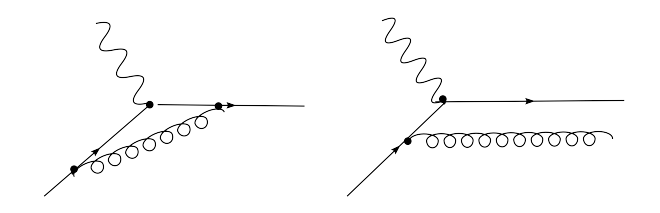
\includegraphics[width=1.0\textwidth]{figures/radiative-corrections}
  \caption{Examples of first-order radiative corrections to the quark-photon vertex.}
  \label{fig:radiative-corrections}
\end{figure}

Figure \ref{fig:radiative-corrections} illustrates two first-order gluonic
corrections to the quark-photon vertex. The diagrams contain collinear
divergences due to the massless quarks, so the size of each correction is
actually infinite. The standard technique for dealing with these infinities is
to factorize the reaction into a hard part calculable in perturbative QCD and a
soft part which must be parameterized from experimental observations. Generally
speaking, one encounters terms of the form
%
\begin{equation}
  \alpha_s~ln \frac{Q^2}{m_q^2} = \alpha_s~ln \frac{Q^2}{\mu^2} + \alpha_s~ln \frac{\mu^2}{m_q^2}.
\end{equation}
%
The first term on the right is included in the hard part of the interaction and
the second (infinite) term is absorbed into the parton distribution functions.
The factorization scale \(\mu^2\) is an arbitrary number, and exact physical
results cannot depend on it, but since perturbative results are never exact the
particular choice of scale is important. A common choice is
\(\mu^2 = Q^2\), which means that perfect Bjorken scaling of the distribution
functions is broken; that is \(q(x) \rightarrow q(x,Q^2)\). However, the
dependence on \(Q^2\) is only logarithmic and is calculable by a set of
evolution equations which are presented later.

QCD factorization is completely general and not limited only to higher-order
corrections to DIS. Consider the case of mid-rapidity pion production at a high
energy proton-proton collider. The factorization theorem allows one to write the
hadronic cross section for this process as a convolution of several independent
entities: PDFs describing the probability of picking out a given parton from
each proton, a hard partonic cross section, and a fragmentation function giving
the probability that an outgoing quark will fragment into a pion with a fraction
\(z\) of the parton's momentum. To wit:
%
\begin{equation}
  \sigma_{p_A+p_B \rightarrow \pi+X} = \sum_{a,b,c} f_a(x_A, Q^2) \otimes f_b(x_B, Q^2) \otimes \sigma_{a+b \rightarrow c + X} \otimes D_c^{\pi}(z)
  \label{eqn:factorization}
\end{equation}
%
The sum is over all parton flavors that contribute to the hadronic cross
section. The \(f_i\) are the parton distribution functions; \(D_c^{\pi}(z)\) is
the pion fragmentation function for quark flavor \(c\). The partonic cross
section is calculable using perturbative QCD when the \(Q^2\) of the interaction
is large, while the PDFs and FFs must be parameterized from experimental
results. Fortunately, those distribution functions are \textit{universal}; they
can be measured in any process (commonly \(e^+e^-\) collisions) and then applied
in the calculation of any other cross section. % TODO burton has a statement about the applicability of factorization in DIS and pp->jets with 2 references here

\subsection{Anomalous gluonic contribution to $\Gamma_1$}

A particularly interesting QCD correction to DIS is shown in Figure
\ref{fig:box-diagram}. This correction involves the gluonic version of the Adler
\cite{Adler:1969gk} and Bell and Jackiw \cite{Bell:1969ts} anomalous triangle
diagram, and results in a gluonic contribution to the flavor singlet matrix
element\footnote{This result is only valid in the \(AB\) and \(JET\)
renormalization schemes. In the \(\overline{MS}\) scheme, where \(\Delta
\Sigma\) itself varies with \(Q^2\), the gluonic contribution to \(a_0\) is
zero.}:
%
\begin{equation}
  a_0(Q^2) = \Delta \Sigma_q - 3\frac{\alpha_s(Q^2)}{2\pi} \Delta G(Q^2)
  \label{eqn:qcd-a0}
\end{equation}
%
This result invalidates the simple parton model formula \ref{eqn:su3-dis} for
\(a_0\) in terms of the quark spins. In the QCD enhanced parton model, a small
measured value of \(\Gamma_1^p\) (and thus a small \(a_0\)) does not necessarily
imply small quark polarization in the proton.

\begin{figure}
  \centering
  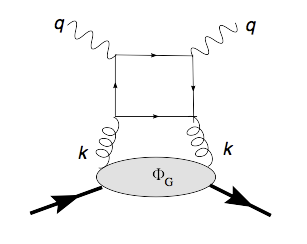
\includegraphics[width=0.5\textwidth]{figures/box-diagram}
  \caption{QCD diagram leading to the anomalous gluon contribution}
  \label{fig:box-diagram}
\end{figure}

\subsection{Spin Sum Rules}

The formulation in \ref{eqn:qcd-a0} has the attractive property that \(\Delta \Sigma_q\) is independent of \(Q^2\) and can be thought of as the quark helicity contribution even in the static (\(Q^2 \rightarrow 0\)) limit. Working in the light-cone gauge, one can write a sum rule for the proton spin which takes the form \cite{Hagler:1998kg, Harindranath:1998ve, Bashinsky:1998if}
%
\begin{equation}
  \frac{1}{2} = \frac{1}{2}\Delta \Sigma_q + \Delta G + L_q + L_g.
  \label{eqn:jaffe-sum-rule}
\end{equation}
%
Unfortunately, the last two terms are not experimentally accessible.  Lattice QCD can measure angular momentum contributions to the proton spin, but it does so in a different gauge and the sum rule \ref{eqn:jaffe-sum-rule} is not gauge invariant.

There exists an alternative sum rule \cite{Jaffe1990509, Ji:1996ek}
%
\begin{equation}
  \frac{1}{2} = \frac{1}{2}\Delta \Sigma_q + \hat{L}_q + \hat{J}_g
\end{equation}
%
where \(\hat{L}_q\) and \(\hat{J}_g\) correspond roughly to the orbital angular momentum of quarks and the total angular momentum of gluons in the nucleon. \(\hat{J}_q = \frac{1}{2}\Delta \Sigma + \hat{L}_q\) is measurable using deeply virtual Compton scattering, and \(\hat{J}_g\) can then in principle be obtained through the evolution of \(\hat{J}_q\).

The subtleties involved in decomposing the spin of the proton into experimental observables should not be viewed as a deterrent towards further experiments.  On the contrary, they are an opportunity for the data to lead the way to greater insight.


\section{Access to $\Delta G$}

The polarized gluon density affects a affects a wide variety of observables,
and a rich experimental and computational program has developed over the past
few decades to strictly constrain it. The first experimental constraints on
\(\Delta G\) were obtained through measurements of the variation with \(Q^2\)
at fixed \(x\) of the \(g_1\) structure functions, while more recent
measurements in polarized DIS have focused on the photon-gluon fusion channel
that is directly sensitive to polarized glue. The results in this thesis rely
on a complementary and unique experimental program of polarized proton
collisions, where the partonic interactions frequently involve one or more
gluons in the initial state.

\subsection{Scaling Violations in parton densities}

QCD introduces a \(Q^2\) dependence into the parton distribution functions which is calculable using the evolution equations
%
\begin{eqnarray}
  \frac{d~\Delta q(x,Q^2)}{d~ln Q^2} &=& \frac{\alpha_s}{2 \pi} \left[ \Delta P_{qq} \otimes \Delta q + \Delta P_{qg} \otimes \Delta g \right], \nonumber \\
  \frac{d~\Delta g(x,Q^2)}{d~ln Q^2} &=& \frac{\alpha_s}{2 \pi} \left[ \Delta P_{gq} \otimes \Delta q + \Delta P_{gg} \otimes \Delta g \right].
\end{eqnarray}
%
The \(\Delta P\) are polarized splitting functions calculated perturbatively in \(\alpha_s\).  The original parton model equation for \(g_1\) \ref{eqn:simple-g1} becomes
%
\begin{equation}
  g_1(x, Q^2) = \frac{1}{2} \sum_{j} e_j^2 \left[\Delta q_j^2 + \Delta \bar{q}_j^2 + \frac{\alpha_s}{2 \pi} \left(\Delta C_j \otimes \left[\Delta q_j + \Delta \bar{q}_j\right] + \Delta C_g \otimes \Delta g\right)\right].
  \label{eqn:enhanced-g1}
\end{equation}
%
where the sum is over flavors and the \(\Delta C_j\) are Wilson coefficients. Given measurements of \(g_1\) at a fixed value of \(x\) and varying \(Q^2\), one can use \ref{eqn:enhanced-g1} to solve for the polarized gluon density. The  technique has proven very effective in unpolarized DIS, where a mix of fixed-target and collider data provides precise measurements of the structure functions across five decades in \(Q^2\) --- an excellent ``lever arm'' for the evolution equations.  In contrast, Figure \ref{fig:g1-versus-q2} plots the current world data on \(g_1\).  Extractions of \(\Delta g(x)\) from these fixed-target data are prone to significant uncertainties.  An example analysis from Leader, Sidorov, and Stamenov is shown in Figure \ref{fig:g1-deltag}; in that analysis, even the sign of the gluon polarization is not constrained by the data. The proposed Electron Ion Collider (EIC), a polarized analogue to HERA, would augment the current data on \(g_1\) with a broad range of high \(Q^2\) measurements and thus dramatically improve the constraints on polarized structure functions obtained through \(g_1\) evolution.

\begin{figure}
  \centering
  \includegraphics[width=0.7\textwidth]{figures/g1_x_q2}
  \caption{World data on the $g_1$ structure functions of the proton, plotted
  versus $Q^2$ for several values of $x$. An analysis of the variation with
  $Q^2$ yields a parameterization of the polarization gluon distribution.}
  % http://www2.lns.mit.edu/eic/Bruell.pdf
  \label{fig:g1-versus-q2}
\end{figure}

\begin{figure}
  \centering
  \includegraphics[width=0.6\textwidth]{figures/lss06_deltag}
  \caption{Extraction of the polarized gluon distribution from an analysis of
  scaling violations in DIS and SIDIS. The gray band indicates statistical and
  systematic uncertainties summed in quadrature. Analyses assuming positive,
  negative, and sign-changing gluon polarization all resulted in a comparable
  goodness-of-fit \cite{Leader:2006xc}}
  \label{fig:g1-deltag}
\end{figure}

\subsection{Photon-Gluon Fusion}

Given the relatively small lever arm in $Q^2$ currently available to constrain
$\Delta G$ via evolution of $g_1$, it is natural to pursue an alternative
approach involving observables that are directly linked to the gluon
polarization. In photon-gluon fusion (PGF), the lepton emits a real or virtual
photon that interacts with a gluon radiated from the nucleon to produce a
$q\bar{q}$ pair (see Figure \ref{fig:pgf}). PGF is a rare process compared to
scattering off of quarks in the nucleon, and as such analyses need a way to
enhance the signal to background ratio. The golden signature for PGF is charm
in the final state, since the nucleon itself has a negligible charm content.
Charm production has a small cross section, so analyses that look for
high-$p_T$ final states are also common.

Figure \ref{fig:pgf-deltag} summarizes results for the gluon polarization
extracted at leading order from analyses of photon-gluon fusion processes.
SMC, HERMES, and COMPASS have all released results based on the detection of
high-$p_T$ hadrons or jets, and COMPASS has released a single data point from
an analysis of charmed ($D^0$ and $D^*$) mesons. The data cover an $x$ range
of approximately $0.07 < \langle x \rangle < 0.2$ and restrict the magnitude
of the gluon polarization within that region. No NLO analysis of PGF data on
$\Delta G$ is currently available.

\begin{figure}
  \centering
  \begin{fmfgraph*}(200,150)
    \fmfleft{proton,gamma}
    \fmfright{proton',quark1,quark2}
    \fmf{fermion,width=2.5}{proton,v1}
    \fmf{fermion}{v1,proton'}
    \fmf{gluon}{v1,v2}
    \fmfblob{.15w}{v1}
    \fmf{fermion}{v2,quark1}
    \fmf{fermion}{v2,v3,quark2}
    \fmf{photon}{gamma,v3}

    % wow, it really feels like I should not have to do all of this
    \fmffixedx{0.}{v2,v3}
    \fmffixedy{0.}{v2,quark1}
    \fmffixedy{0.}{v3,quark2}
    \fmffixedy{0.}{v1,proton'}
    \fmffreeze
    \fmfshift{(0,-0.2h)}{v3}
    \fmfshift{(0.09w,-0.2h)}{quark2}
    \fmfshift{0,0.15h}{v1,proton'}
    
    % finally, add lines for outgoing quarks in struck proton
    \fmfi{plain}{vpath (__v1, __proton') shifted (thick*(-0.5,3.5))}
    \fmfi{plain}{vpath (__v1, __proton') shifted (thick*(-0.5,-3.5))}
  \end{fmfgraph*}
  \caption{Feynman diagram of photon-gluon fusion process}
  \label{fig:pgf}
\end{figure}


\begin{figure}
  \centering
  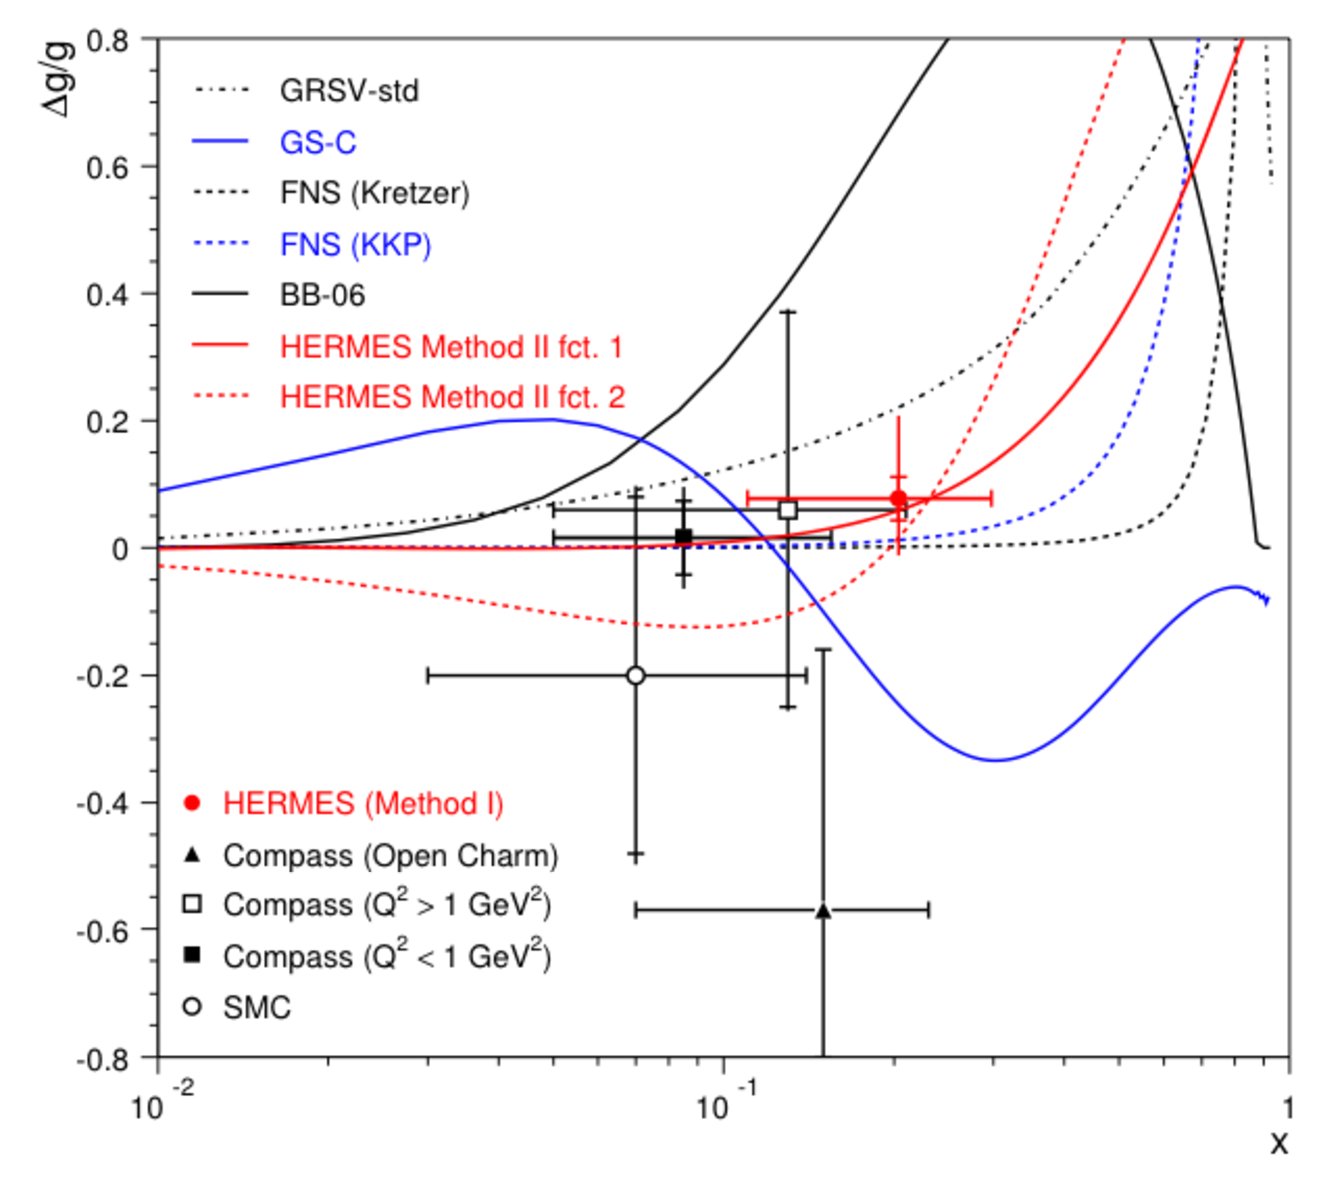
\includegraphics[width=0.7\textwidth]{figures/dgg-hermes-final}
  \caption{Compilation of $\Delta g(x)/g(x)$ measurements from SMC, HERMES,
  and COMPASS plotted versus momentum fraction \cite{Hasch:2009zza}.}
  \label{fig:pgf-deltag}
\end{figure}

% ... this is wrong, the number is just for the COMPASS open charm measurement, the most recent LO global analysis from COMPASS yields $\Delta g(x)/g(x) = -0.49~\pm~0.27~(stat)~\pm~0.11~(syst)$ at a scale $\mu^2 \sim 13~(GeV/c)^2$ and at an average gluon momentum fraction $\langle x \rangle ~\sim 0.11$ \cite{Alekseev:2009ey}.

%% Direct \Delta G figure without preliminary results
% \begin{figure}
%   \includegraphics[width=1.0\textwidth]{figures/compass_deltag}
%   \caption{\cite{Alekseev:2009ey}}
% \end{figure}

\subsection{Polarized Proton Collisions}

DIS is an electromagnetic process, so the techniques used to study the polarized gluon distribution in that environment must rely on higher-order QCD effects. In contrast, collisions of polarized protons are usually mediated by the strong force. Spin-dependent observables in these collisions are  directly sensitive to the polarized gluon content, as a significant fraction of hard scatterings contain one or more gluons in the initial partonic state. A given observable's particular sensitivity to polarized glue is calculable thanks to the triumvirate of asymptotic freedom, factorization, and PDF universality.  As of this writing, calculations performed at next-to-leading order (NLO) are the state of the art.

\begin{figure}\begin{center}
  \includegraphics[width=0.5\textwidth]{figures/partonic_asymmetry}
  \caption{Lowest-order analyzing powers for various partonic subprocesses
  present in polarized proton collisions \cite{Bunce:2000uv}.}
  \label{fig:partonic-asymmetries}
\end{center}\end{figure}

In principle one could directly measure a polarized cross section, e.g. a polarized analogue to \ref{eqn:factorization}.  In practice, a more precise result is obtained through asymmetry measurements that use the ratio of polarized and unpolarized cross sections to cancel out several sources of spin-independent uncertainty present in the absolute cross section measurements.  The observable of primary interest in this work is \(A_{LL}\), defined for inclusive pion production as
%
\begin{equation}
  A_{LL}(\pi + X) = \sum_{a,b,c} \frac{\Delta f_a(x_A, Q^2) \otimes \Delta f_b(x_B, Q^2) \otimes \left[ \hat{a}_{LL}^{ab \rightarrow cX} \sigma_{ab \rightarrow cX} \right] \otimes D_c^{\pi}(z)}{f_a(x_A, Q^2) \otimes f_b(x_B, Q^2) \otimes \sigma_{ab \rightarrow cX} \otimes D_c^{\pi}(z)}.
\end{equation}
%
\(\hat{a}_{LL}^{ab \rightarrow cX} \equiv \Delta \sigma_{ab \rightarrow cX} / \sigma_{ab \rightarrow cX}\) is the asymmetry of the underlying partonic hard scattering.  Figure \ref{fig:partonic-asymmetries} plots partonic asymmetries calculated using perturbative QCD for common subprocesses.  \(A_{LL}\) for charged pion production integrates over all five of these subprocess asymmetries.

\(A_{LL}\) can be measured and interpreted in a perturbative QCD context for a wide variety of final states. This thesis presents results on \(A_{LL}\) for inclusive charged pion production, as well as for charged pions produced azimuthally opposite an identified jet.  Figure \ref{fig:all-predictions} shows the effect of polarized glue on these observables.  The curves represent asymmetries calculated perturbatively at NLO assuming various polarized gluon distributions, ranging from an unpolarized glue (GRSV ZERO) to extreme fully-polarized scenarios (GRSV MIN).  The STD scenario in the GRSV \cite{Gluck:2000dy} set represented a best-fit extraction of polarized structure functions from \(g_1\) evolution data at the time of its release, while Gehrmann and Stirling's ``Set C'' \cite{Gehrmann:1995ag} is a scenario in which gluons are strongly polarized at low \(x\) but the overall integral of the gluon polarization is small thanks to a node in the distribution function.  Finally, the DSSV \cite{deFlorian:2008mr} set of structure functions is the first to incorporate data from measurements of \(A_{LL}\), specifically the inclusive \(\pi^0\) channel at PHENIX and the inclusive jet channel at STAR.  The measurements in this thesis can be included in a future update to the DSSV set and other similar global analyses in order to directly inform our understanding of the polarized gluon distribution.


\begin{figure}
  \subfloat{
    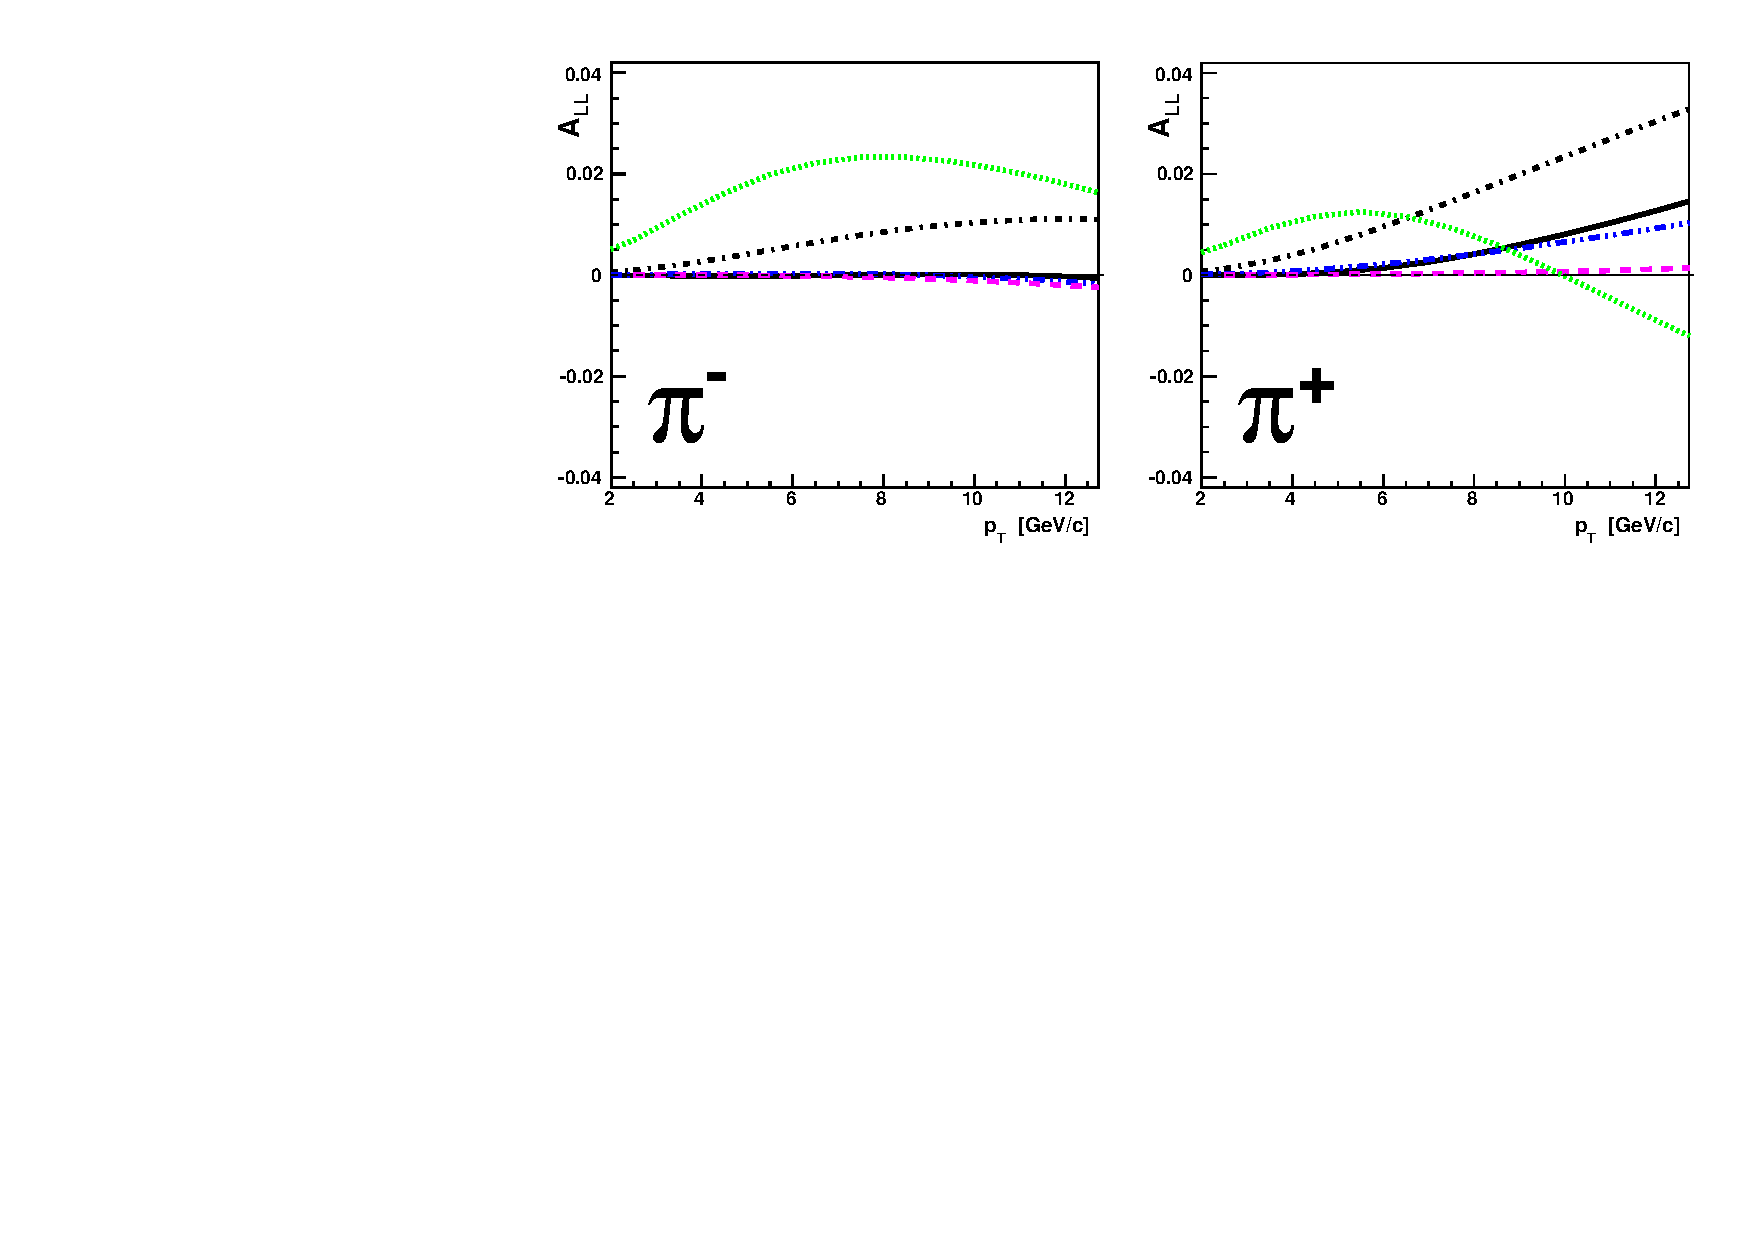
\includegraphics[width=1.0\textwidth]{figures/inclusive_predictions}
  }
  \newline
  \subfloat{
    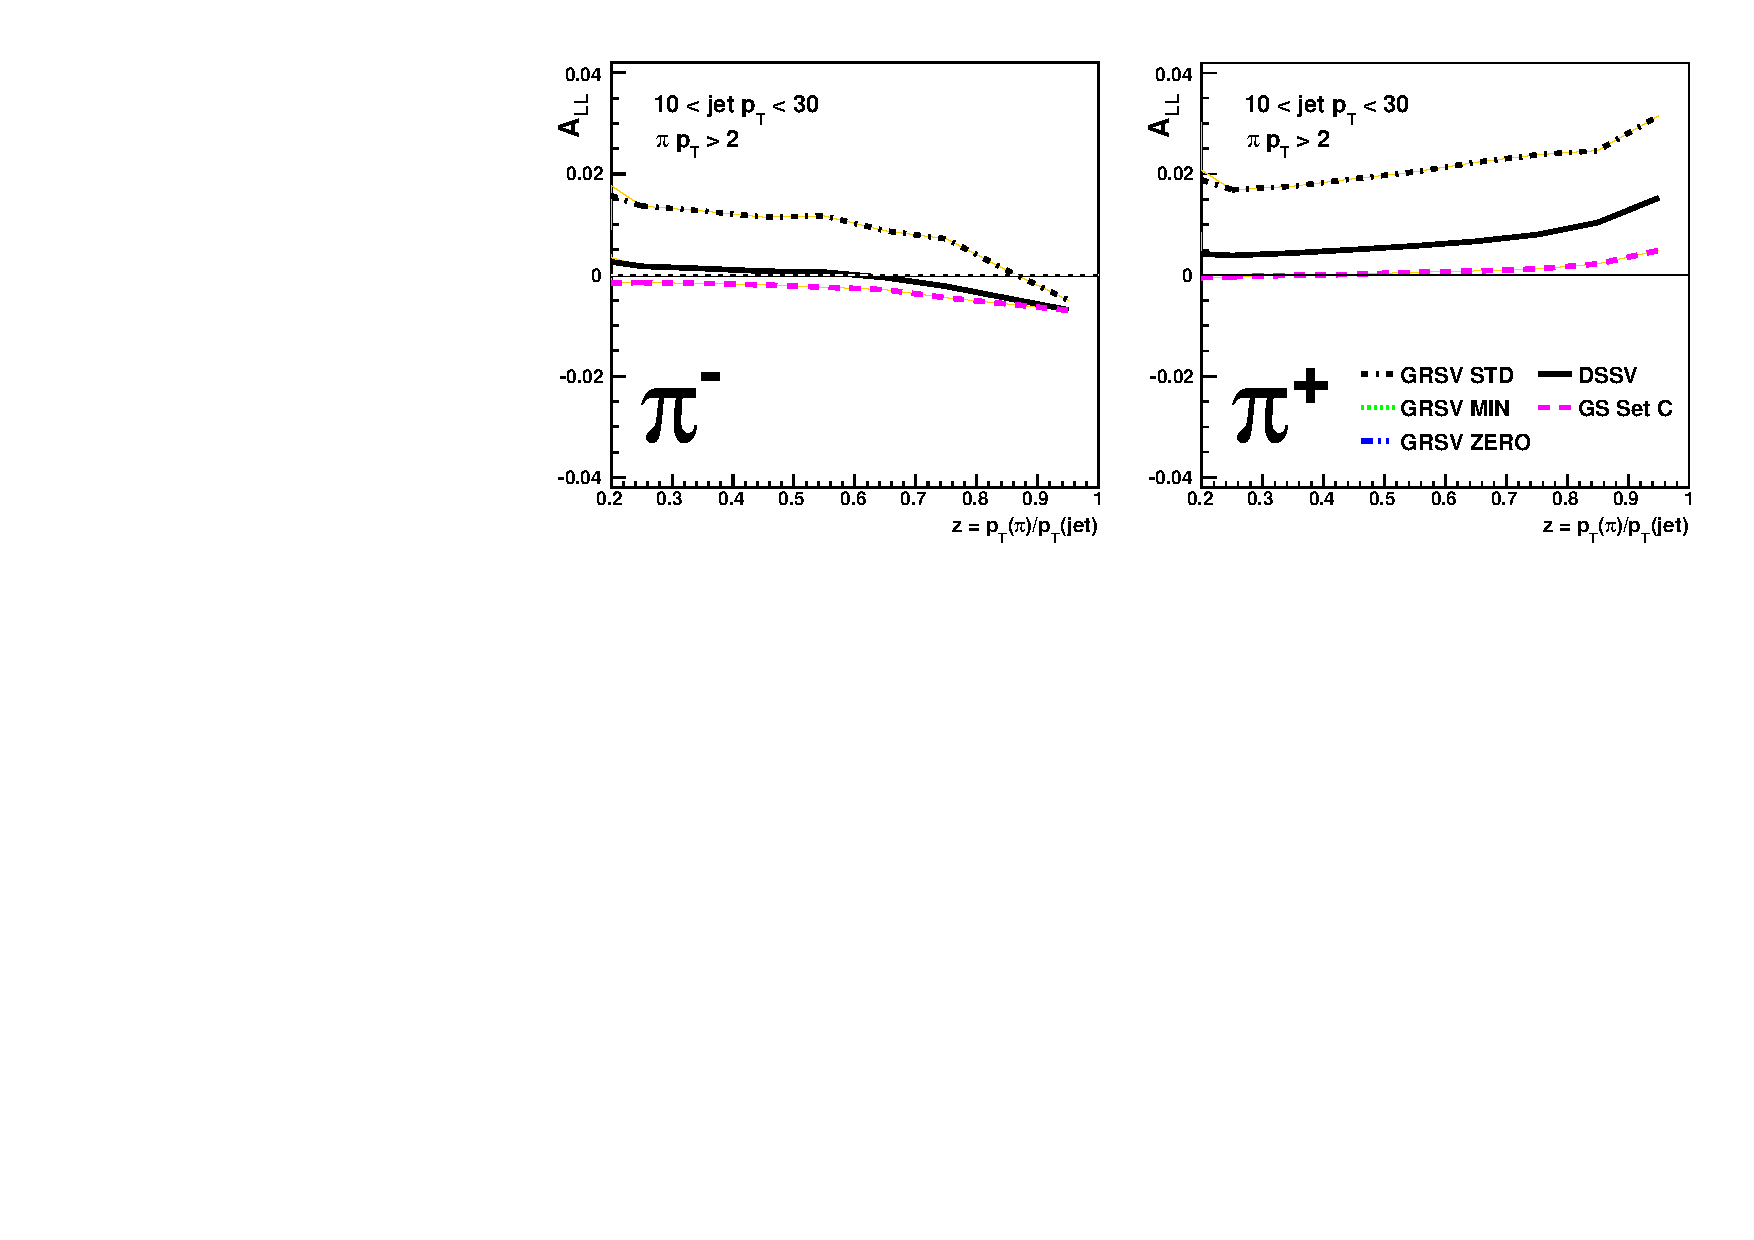
\includegraphics[width=1.0\textwidth]{figures/jet_pion_predictions}
  }
  \caption{Predictions for $A_{LL}$ assuming various input distributions for the gluon polarization \cite{Gluck:2000dy, Gehrmann:1995ag, deFlorian:2008mr}. The pion fragmentation functions can be found in \cite{deFlorian:2007nk}, and the NLO calculation was performed in the purely inclusive case by J\"ager et al. \cite{Jager:2002xm}, and in the jet + pion case by de Florian \cite{deFlorian:2009fw}.}
  \label{fig:all-predictions}
\end{figure}

